\documentclass[tikz]{standalone}

\usepackage{amsmath}
\usepackage{physics}

\usetikzlibrary{arrows.meta,positioning}

\begin{document}
	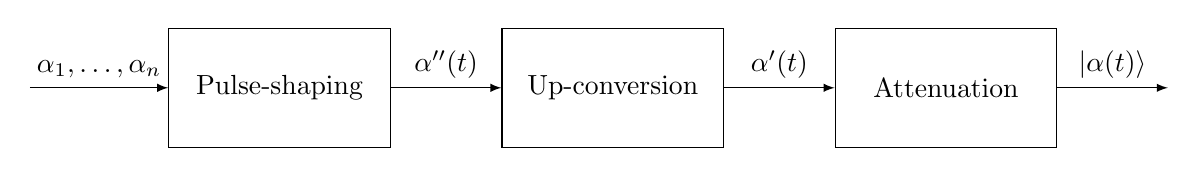
\begin{tikzpicture}[
		node distance=4em,
		arrow/.style={-latex},
		block/.style={draw, minimum height=10ex, minimum width=8em, align=center},
	]
		\coordinate (in) at (0,0);
		\node (ps) [block, right=5em of in] {Pulse-shaping};
		\node (uc) [block, right=of ps] {Up-conversion};
		\node (at) [block, right=of uc] {Attenuation};
		\coordinate[right=of at] (out);
		
		\draw[arrow] (in) -- node[above]{$\alpha_1,\dots,\alpha_n$} (ps);
		\draw[arrow] (ps) -- node[above]{$\alpha^{\prime\prime}(t)$} (uc);
		\draw[arrow] (uc) -- node[above]{$\alpha^{\prime}(t)$} (at);
		\draw[arrow] (at) -- node[above]{$\ket{\alpha(t)}$} (out);
	\end{tikzpicture}
\end{document}
